%!TEX root = causalityRetweetPropensity.tex

\section{Discovering Causal Structure}
\begin{itemize}
\item motivation
\item data
\item method
\item findings
\end{itemize}


As discussed above, our goal is to identify the variables that cause or influence retweet propensity. The variables that we consider in this work are friends count, status count, followers count, klout score and sentiment. As a first step, we need to identify if there is any causal structure involving  these variables and retweets. We use the PC algorithm described in the next section. 
\subsection{Dataset}
A random sample of about 1 million tweets are used for determining the causal graph structure. 
\subsection{The PC Algorithm}
The PC (Peter Spirtes, Clark Glymour) algorithm is based on two assumptions: Causal Markov Property and Causal Faithfulness. Consider a graph consisting of variables \{X,Y, Z, Z1,Z2...\}. Given the data, the PC algorithm tries to come up with the causal graph structure. The PC algorithm has two main steps. In the first step, from the data, it learns a skeleton graph, i.e., a graph with only undirected edges. As a second step, it orients the undirected edges to form a markov equivalence class of DAGs. PC algorithm is based on the fact that, if there is no edge between variables A and B, then there is a set of vertices C either connected to A or B such that A is independent of B, conditioned on C, or C d-separates A and B. \\
• For each X and Y, see if X is independent of Y; if so, remove their edge.
• For each X and Y which are still connected, and each third variable Z, see if
X is independent of Y given \{Z\}; if so, remove the edge between X and Y.
• For each X and Y which are still connected, and each third and fourth variables
Z1 and Z2, see if X is independent of Y given \{Z1,Z2\}; if so, remove their edge.

\subsection{Our findings}

\begin{center}
\begin{figure}
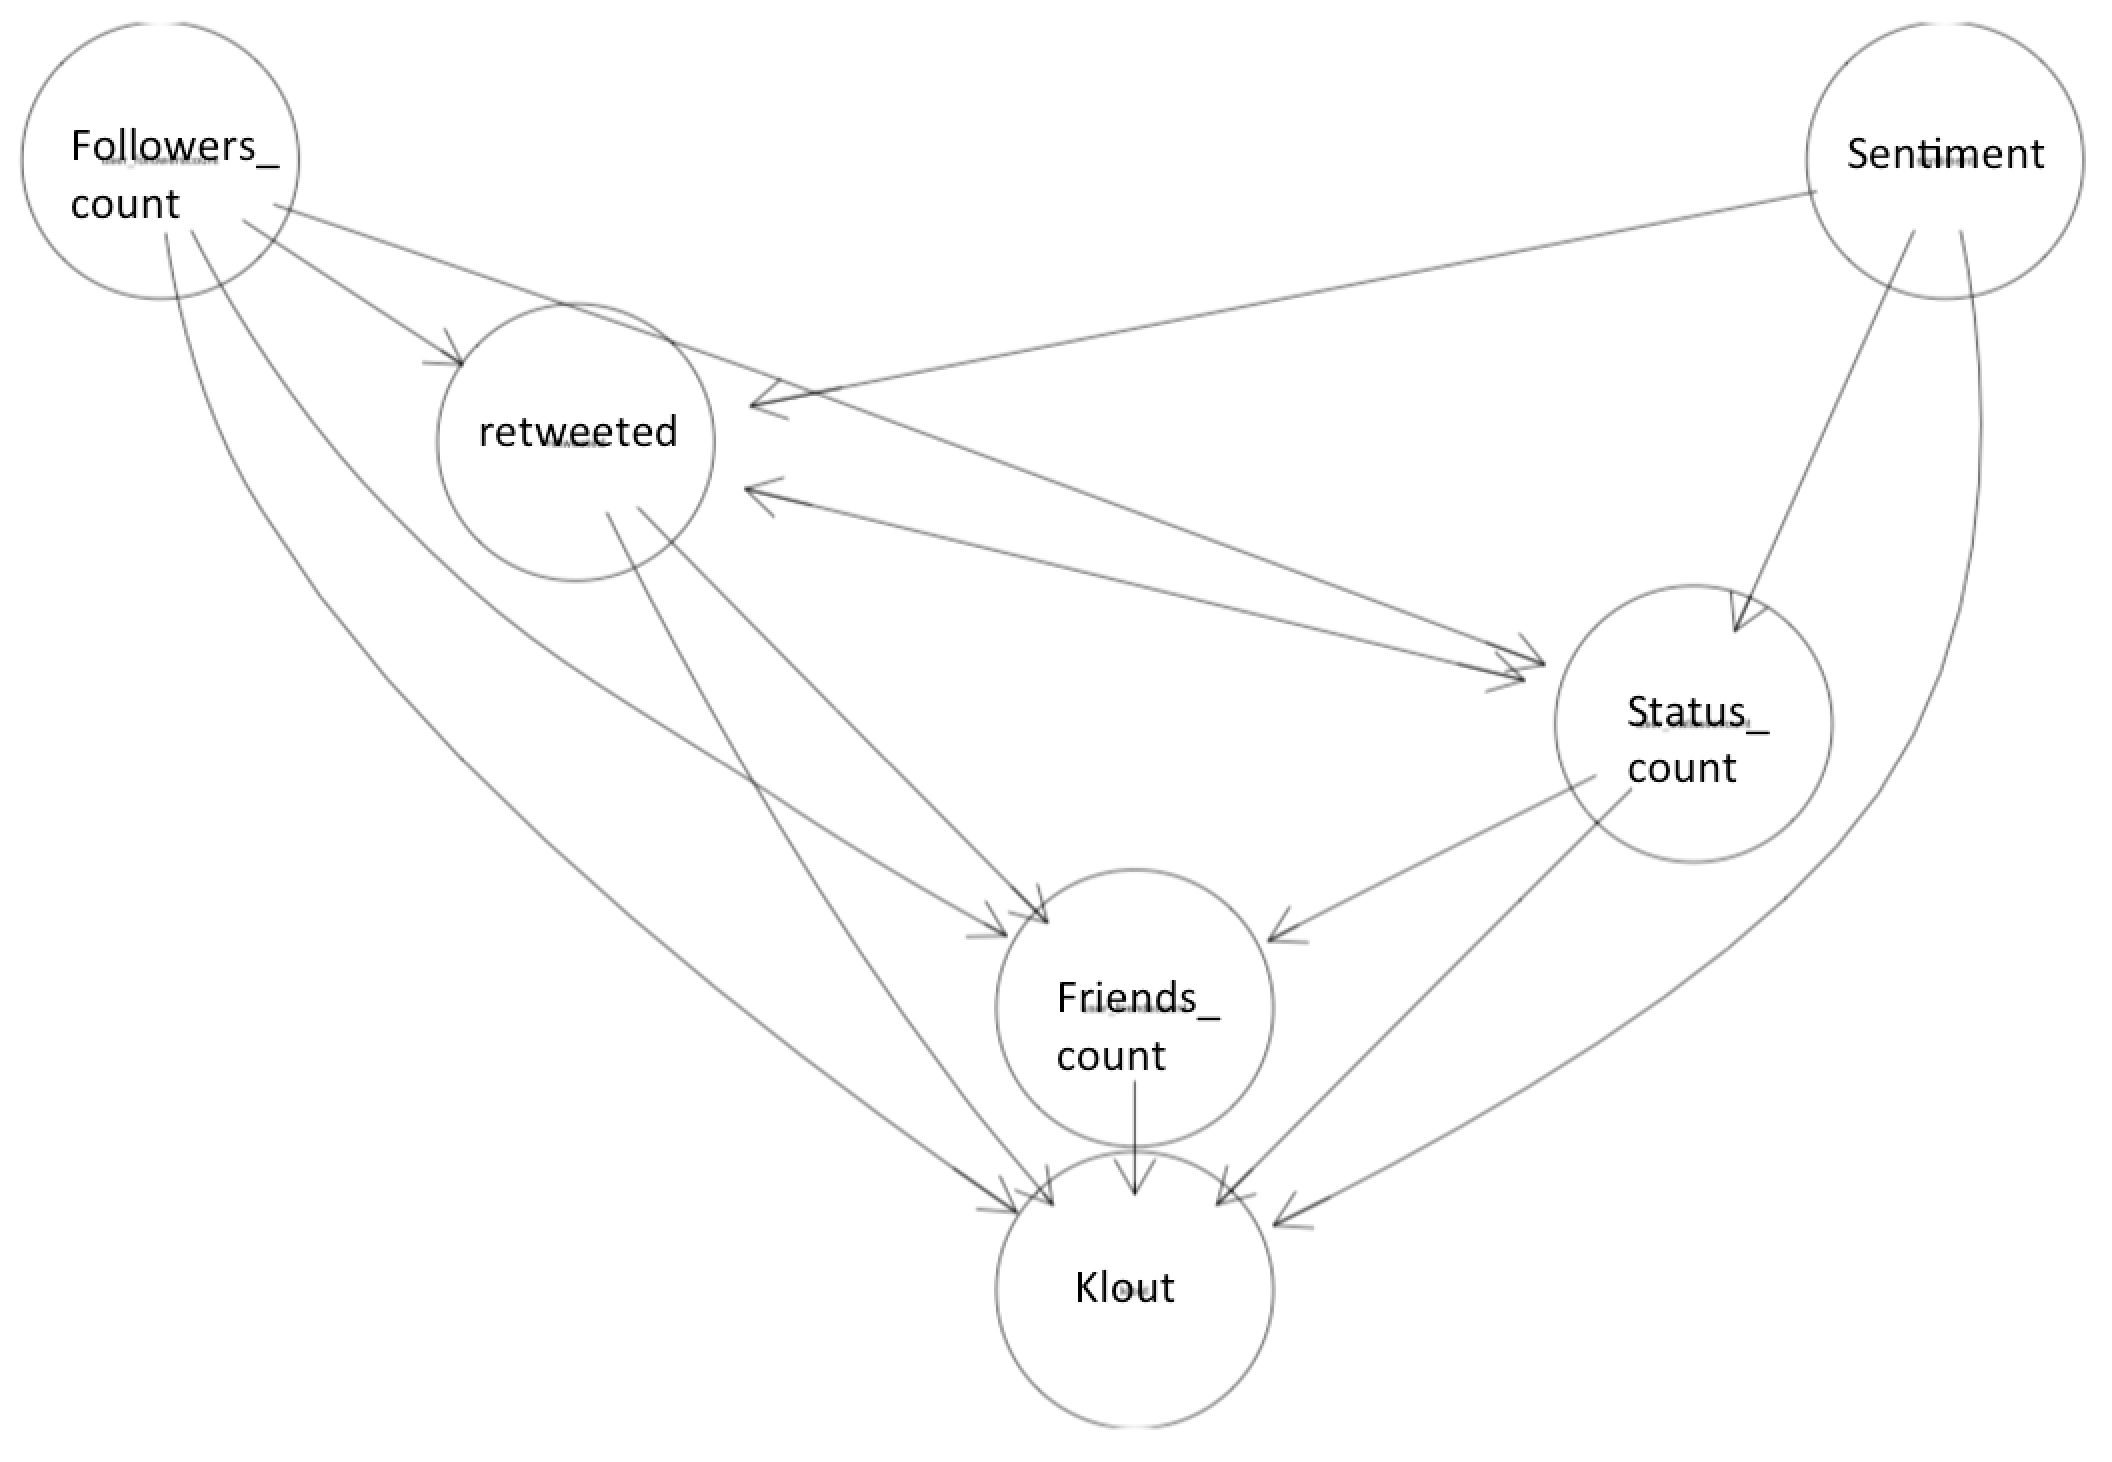
\includegraphics[scale=0.2]{pc}
\caption{Output from the PC algorithm}
\end{figure}
\end{center}

